\documentclass[border=5pt]{standalone}
    \usepackage{tikz}
    \usetikzlibrary{arrows.meta}
    \begin{document}
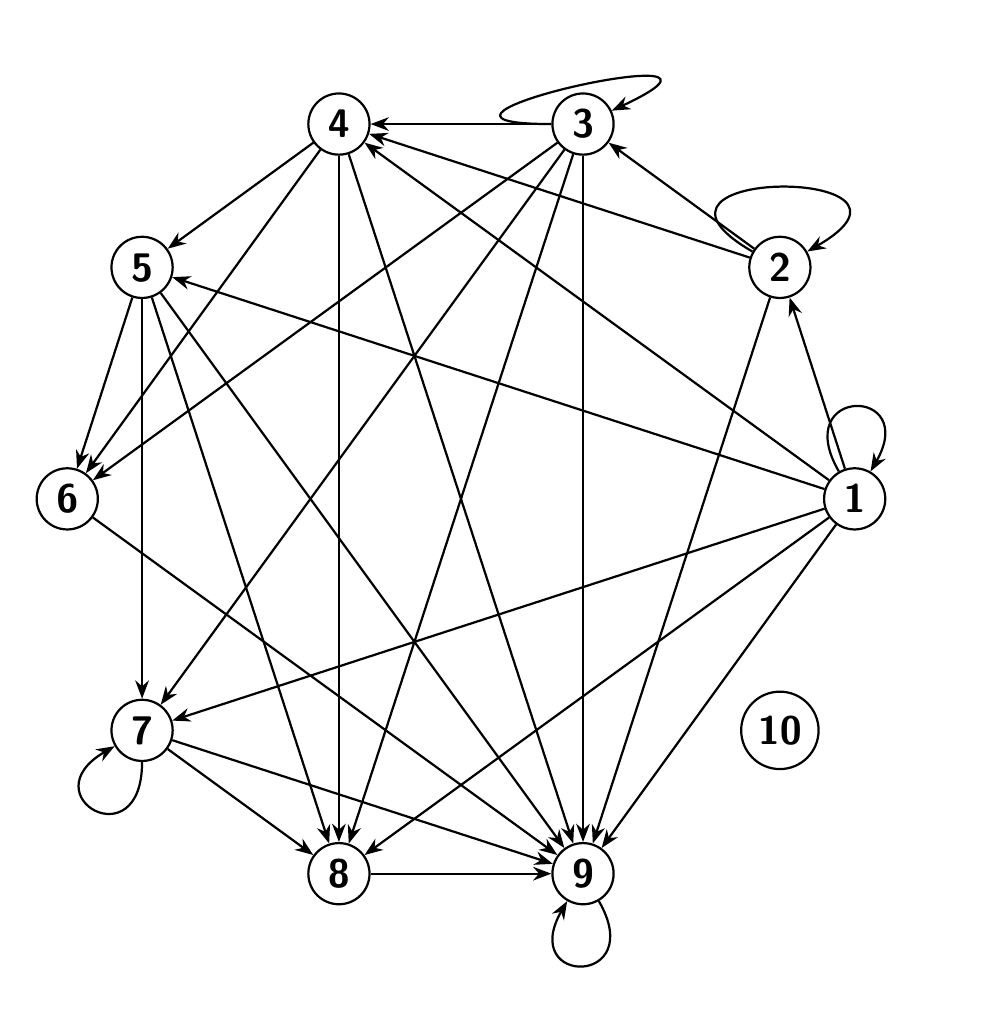
\begin{tikzpicture}[->, >=Stealth, auto, node distance=2.5cm, thick,
	main node/.style={circle, draw, font=\sffamily\Large\bfseries}]
	
	% Nodes arranged in a circle
	\node[main node] (1) at (5.00,0.00) {1};
	\node[main node] (2) at (4.05,2.94) {2};
	\node[main node] (3) at (1.55,4.76) {3};
	\node[main node] (4) at (-1.55,4.76) {4};
	\node[main node] (5) at (-4.05,2.94) {5};
	\node[main node] (6) at (-5.00,0.00) {6};
	\node[main node] (7) at (-4.05,-2.94) {7};
	\node[main node] (8) at (-1.55,-4.76) {8};
	\node[main node] (9) at (1.55,-4.76) {9};
	\node[main node] (10) at (4.05,-2.94) {10};
	
	% Edges with adjusted loops
	\path (1) edge[out=120, in=60, looseness=8] (1);  % Top loop for node 1
	\path (2) edge[out=150, in=30, looseness=8] (2);  % Top-right loop for node 2
	\path (3) edge[out=180, in=25, looseness=8] (3);    % Top loop for node 3
	\path (7) edge[out=270, in=210, looseness=8] (7);  % Bottom-left loop for node 7
	\path (9) edge[out=300, in=240, looseness=8] (9);  % Bottom-right loop for node 9
	
	% Regular edges
	\path (1) edge (7);
	\path (1) edge (4);
	\path (1) edge (8);
	\path (1) edge (2);
	\path (1) edge (9);
	\path (1) edge (5);
	\path (2) edge (4);
	\path (2) edge (3);
	\path (2) edge (9);
	\path (3) edge (4);
	\path (3) edge (7);
	\path (3) edge (6);
	\path (3) edge (9);
	\path (3) edge (8);
	\path (4) edge (5);
	\path (4) edge (6);
	\path (4) edge (9);
	\path (4) edge (8);
	\path (5) edge (7);
	\path (5) edge (9);
	\path (5) edge (6);
	\path (5) edge (8);
	\path (6) edge (9);
	\path (7) edge (9);
	\path (7) edge (8);
	\path (8) edge (9);
\end{tikzpicture}
    \end{document}